\documentclass[11pt,a4paper]{article}
\usepackage[margin=1in]{geometry}
\usepackage[T1]{fontenc}
\usepackage[utf8]{inputenc}
\usepackage{lmodern}
\usepackage{hyperref}
\usepackage{enumitem}
\usepackage{array}
\usepackage{longtable}
\usepackage{booktabs}
\usepackage{xurl}
\usepackage{tikz}
\usepackage{float}
\usetikzlibrary{arrows.meta, positioning, shapes.geometric}

\hypersetup{colorlinks=true,linkcolor=blue,urlcolor=blue}
\newcommand{\codepath}[1]{\path{#1}}
\setlength{\tabcolsep}{4pt}
\renewcommand{\arraystretch}{1.15}
\tikzset{
  box/.style={rectangle, draw, rounded corners, align=center, inner sep=3pt, minimum width=36mm},
  decision/.style={diamond, draw, aspect=2.2, align=center, inner sep=2pt},
  line/.style={-Latex}
}

\title{Phase-0 Trace Utilization Validation\\
\large How Tenstorrent Baseline Logic is Carried into Phase-1 and Phase-2}
\author{SIT Engine Architecture}
\date{\today}

\begin{document}
\maketitle
\tableofcontents
\newpage

\section{Purpose}
This document explains, in validation terms, how the Phase-0 Tenstorrent baseline is used in the project:
\begin{itemize}[leftmargin=*]
  \item which baseline semantics were carried forward,
  \item where those semantics are implemented in Phase-1 and Phase-2,
  \item how golden validation enforces that behavior remains stable.
\end{itemize}

The intent is to show that Phase-0 influence is not limited to trace-format conversion; it is a behavioral contract that gates engine correctness.

\section{Baseline Provenance and Anchor Artifacts}
\subsection*{Verified Phase-0 Baseline Context}
\begin{itemize}[leftmargin=*]
  \item Source repo: \url{git@github.com:Srinidhi-Magesh08/Tenstorrent_test_raw_files.git}
  \item Baseline branch/commit: \texttt{main} @ \texttt{4512ce4e1a689f64c866160bf1f8e7e5e3e2ec89}
  \item Baseline run artifact: \codepath{phase0_golden/tt_run_2026-02-09/raw_profiler/profile_log_device.csv}
\end{itemize}

\subsection*{Project Artifacts that Anchor the Baseline}
\begin{itemize}[leftmargin=*]
  \item Phase-0 conversion logic: \codepath{Phase-1/phase0_trace_to_sit.py}
  \item Phase-0-derived sample trace: \codepath{Phase-1/datasets/traces/trace_F_phase0_wormhole_sample.csv}
  \item Pinned expected outputs: \codepath{Phase-1/tests/fixtures/phase0_parity_expected.json}
  \item Parity gate: \codepath{Phase-1/tests/check_phase0_parity.py}
  \item Golden orchestrator: \codepath{Phase-1/tests/run_golden_suite.py}
\end{itemize}

\section{What Logic is Actually Carried Forward}
\subsection*{Core Carry-Forward Semantics}
\begin{enumerate}[leftmargin=*]
  \item \textbf{Event-pair boundary semantics} from profiler zones (\texttt{ZONE\_START}/\texttt{ZONE\_END}) are preserved as half-open intervals.
  \item \textbf{Deterministic ordering at equal timestamps} is preserved (\texttt{ZONE\_END} before \texttt{ZONE\_START}) to prevent boundary artifacts.
  \item \textbf{Cycle-time normalization} is preserved by converting TT cycle timestamps into microseconds with a fixed frequency model.
  \item \textbf{Window boundary policy} is preserved through exact slicing logic (epsilon-adjusted end boundary).
  \item \textbf{Residency-gated accumulation policy} is preserved through interval intersection and resident-time accounting.
  \item \textbf{Deterministic replay expectations} are preserved via fixture-driven parity checks.
\end{enumerate}

\subsection*{Carry-Forward Mapping: Requirement to Enforcement}
\begin{longtable}{@{}>{\raggedright\arraybackslash}p{0.28\textwidth} >{\raggedright\arraybackslash}p{0.30\textwidth} >{\raggedright\arraybackslash}p{0.36\textwidth}@{}}
\toprule
\textbf{Baseline Requirement} & \textbf{Implementation Path} & \textbf{Validation Gate} \\
\midrule
\endhead
Zone boundary pairing must define intervals, not samples &
\codepath{phase0_trace_to_sit.py} parses only \texttt{ZONE\_START}/\texttt{ZONE\_END} and builds interval rows &
Phase-1 parity compares generated windows/summary against pinned expected outputs \\

Equal-time transitions must be deterministic &
Sort key enforces \texttt{ZONE\_END} before \texttt{ZONE\_START} in converter &
Parity + invariant gates fail on drift caused by boundary mis-ordering \\

Cycle domain must map to stable time base &
Converter maps \texttt{time[cycles since reset]} to \texttt{us} using chip frequency and rebases to first timestamp &
Phase-1 parity fixture pins resulting window-level values \\

Window slicing must be boundary-exact &
\codepath{sit_engine_phase1.py} uses epsilon-aware end-window selection &
\codepath{check_invariants.py} and parity checks detect off-by-one window assignment regressions \\

Residency must gate all accumulation &
Engine intersects state intervals with merged residency masks before accumulation &
Mode-specific invariants (\texttt{partial}, \texttt{exact\_boundary}, \texttt{skip\_w0}) enforce gating behavior \\

Output behavior must remain stable release-to-release &
Golden suite requires parity trace execution and runs strict checker &
Suite fails if parity trace not executed or if any value diverges \\
\bottomrule
\end{longtable}

\section{How Validation Uses the Baseline in Each Phase}
\subsection*{Phase-1 (Direct Baseline Parity)}
Phase-1 has a strict numeric parity gate for the Wormhole-derived sample trace:
\begin{enumerate}[leftmargin=*]
  \item Golden suite loads manifest and executes all traces.
  \item For the expected parity trace path, it invokes \codepath{check_phase0_parity.py}.
  \item Checker validates required summary keys, row counts, columns, and per-value comparisons (float tolerance + exact scalar/list checks).
  \item If parity trace is missing from execution or values drift, suite returns non-zero.
\end{enumerate}

\subsection*{Phase-2 (Semantics Forward, Baseline-Style Logic Through Adapters)}
Phase-2 does not run the same Phase-0 fixture directly by default. Instead:
\begin{enumerate}[leftmargin=*]
  \item Platform adapters (Spike/QEMU/gem5) map simulator traces into the same normalized contract expected by the engine.
  \item Marker-driven ON/OFF span logic (\texttt{101..106}) provides explicit residency/stall/idle boundaries equivalent to the event-boundary model.
  \item Golden pipelines call the same engine path (\codepath{sit_engine_phase1.py}) and run invariants on outputs.
\end{enumerate}

This keeps computation semantics centralized while changing only source-specific parsing.

\section{Inspirations Taken Forward from Phase-0}
\subsection*{Design Inspirations that Became Engine/Adapter Policy}
\begin{itemize}[leftmargin=*]
  \item \textbf{Boundary-event worldview:} throughput analysis should be interval-based, not point-sampled.
  \item \textbf{Deterministic replay:} trace-driven evaluation should be reproducible under fixed parameters.
  \item \textbf{Hardware-agnostic core math:} parsing is platform-specific; windowing/SIT computation is platform-neutral.
  \item \textbf{Validation as behavior lock:} parity/invariant gates are mandatory to prevent silent semantic drift.
\end{itemize}

\subsection*{What is Not Claimed}
\begin{itemize}[leftmargin=*]
  \item Phase-2 does not currently claim strict numeric parity to the same Phase-0 fixture unless explicitly wired as an extra gate.
  \item Baseline provenance metadata alone is not validation; parity and invariants are the enforcement mechanisms.
\end{itemize}

\section{Flowchart: End-to-End Logic Carry-Forward}
\begin{figure}[H]
  \centering
  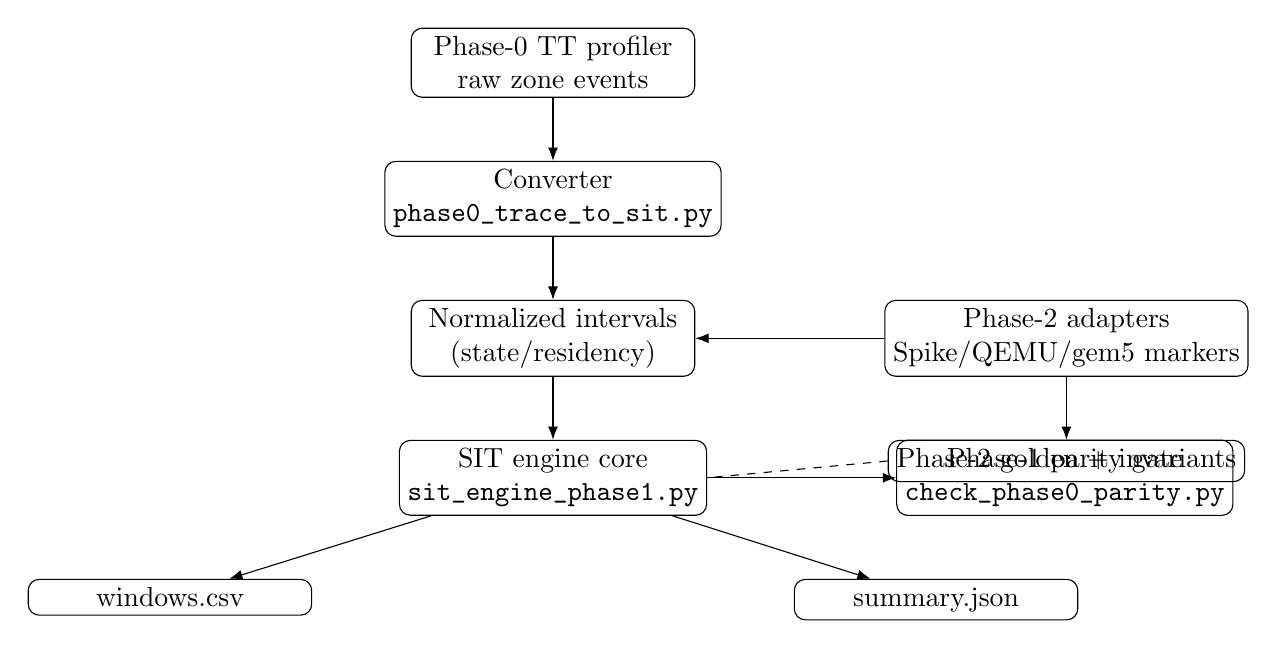
\begin{tikzpicture}[node distance=8mm and 11mm]
    \node[box] (p0) {Phase-0 TT profiler\\raw zone events};
    \node[box, below=of p0] (conv) {Converter\\\codepath{phase0_trace_to_sit.py}};
    \node[box, below=of conv] (norm) {Normalized intervals\\(state/residency)};
    \node[box, below=of norm] (eng) {SIT engine core\\\codepath{sit_engine_phase1.py}};
    \node[box, below left=of eng] (out1) {windows.csv};
    \node[box, below right=of eng] (out2) {summary.json};
    \node[box, right=24mm of eng] (p1v) {Phase-1 parity gate\\\codepath{check_phase0_parity.py}};
    \node[box, right=24mm of norm] (p2a) {Phase-2 adapters\\Spike/QEMU/gem5 markers};
    \node[box, below=of p2a] (p2g) {Phase-2 golden + invariants};

    \draw[line] (p0) -- (conv);
    \draw[line] (conv) -- (norm);
    \draw[line] (norm) -- (eng);
    \draw[line] (eng) -- (out1);
    \draw[line] (eng) -- (out2);
    \draw[line] (eng) -- (p1v);
    \draw[line] (p2a) -- (norm);
    \draw[line] (p2a) -- (p2g);
    \draw[dashed] (p2g.west) -- (eng.east);
  \end{tikzpicture}
  \caption{Baseline Semantics Carried from Phase-0 into Phase-1 and Forward into Phase-2}
\end{figure}

\section{Operational Validation Commands}
\begin{itemize}[leftmargin=*]
  \item Phase-1 golden replay:
\end{itemize}
\noindent\texttt{python tests/run\_golden\_suite.py --outdir /tmp/phase1\_golden\_out}

\begin{itemize}[leftmargin=*]
  \item Direct parity check on the baseline-derived sample:
\end{itemize}
\noindent\texttt{python tests/check\_phase0\_parity.py --windows <windows.csv> --summary <summary.json>}

\begin{itemize}[leftmargin=*]
  \item Phase-2 golden replay (adapter-specific pipelines feed the same engine):
\end{itemize}
\noindent\texttt{python tests/run\_golden\_suite.py --manifest <manifest.json> --outdir <outdir>}

\section{Conclusion}
Phase-0 Tenstorrent traces are utilized as a behavioral reference, not merely a source format:
\begin{itemize}[leftmargin=*]
  \item conversion preserves baseline interval semantics,
  \item engine logic applies deterministic window/residency/SIT computation,
  \item Phase-1 parity and invariants enforce that baseline behavior,
  \item Phase-2 adapters carry forward equivalent semantics into the same engine path.
\end{itemize}

\end{document}
